\subsection{Задача відновлення ваг для графа метелика}
Для зваженого графа метелика ${\bf G}$, зображеного на рисунку \ref{graphMet:image}, розглянемо поставлену задачу.

\begin{figure}[H]
    \centering
    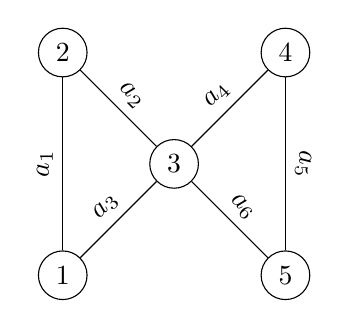
\begin{tikzpicture}[node distance={20mm}, main/.style = {draw, circle}]
    \node[main] (1) {$2$}; 
    \node[main] (2)[below right of=1] {$3$};
    \node[main] (3)[above right of=2] {$4$};
    \node[main] (4)[below right of=2] {$5$};
    \node[main] (5)[below left of=2] {$1$};
    \draw (1) -- node [ above, midway, sloped] {$a_2$}(2);
    \draw (2) -- node [ above, midway, sloped] {$a_4$}(3);
    \draw (3) -- node [ above, midway, sloped] {$a_5$}(4);
    \draw (4) -- node [ above, midway, sloped] {$a_6$}(2);
    \draw (2) -- node [ above, midway, sloped] {$a_3$}(5);
    \draw (5) -- node [ above, midway, sloped] {$a_1$}(1);
    \end{tikzpicture}\\
    \caption{$\bf G$ - граф метелик}
    \label{graphMet:image}
\end{figure}
\textbf{Твердження 3.}\\
Зважений граф метелик можна відновити за такими чотирма підспектрами:$\sigma((4,5)),$ $\sigma((2,3)),$ $\sigma({\bf G}-\{5\}),\ \sigma({\bf G})$.
\begin{figure}[H]
    \centering
     \begin{subfigure}[h]{0.3\linewidth}
        \centering
        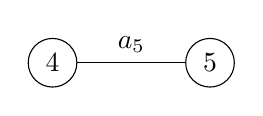
\begin{tikzpicture}[node distance={20mm}, main/.style = {draw, circle}]
            \node[main] (1) {$4$}; 
            \node[main] (2)[right of=1] {$5$};
            \draw (1) -- node [midway, above, sloped] {$a_5$}(2);
        \end{tikzpicture}\\
        \caption{}
        \label{exv1:image}
    \end{subfigure}
    
    \begin{subfigure}[h]{0.3\linewidth}
        \centering
        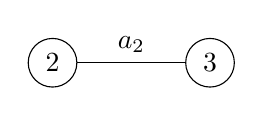
\begin{tikzpicture}[node distance={20mm}, main/.style = {draw, circle}]
            \node[main] (1) {$2$}; 
            \node[main] (2)[right of=1] {$3$};
            \draw (1) -- node [midway, above, sloped] {$a_2$}(2);
        \end{tikzpicture}\\
        \caption{}
        \label{exv1:image}
    \end{subfigure}
    
     \begin{subfigure}[h]{0.3\linewidth}
        \centering
        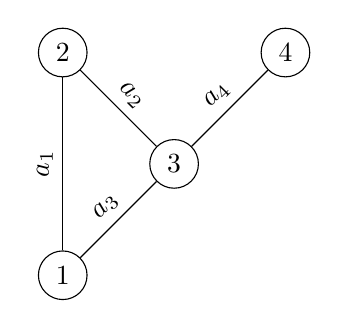
\begin{tikzpicture}[node distance={20mm}, main/.style = {draw, circle}]
            \node[main] (1) {$2$}; 
            \node[main] (2)[below right of=1] {$3$};
            \node[main] (3)[above right of=2] {$4$};
            \node[main] (5)[below left of=2] {$1$};
            \draw (1) -- node [ above, midway, sloped] {$a_2$}(2);
            \draw (2) -- node [ above, midway, sloped] {$a_4$}(3);
            \draw (2) -- node [ above, midway, sloped] {$a_3$}(5);
            \draw (5) -- node [ above, midway, sloped] {$a_1$}(1);
        \end{tikzpicture}\\
        \caption{{\bf G}-\{5\}}
        \label{exv2:image}
    \end{subfigure}
     \begin{subfigure}[h]{0.3\linewidth}
        \centering
        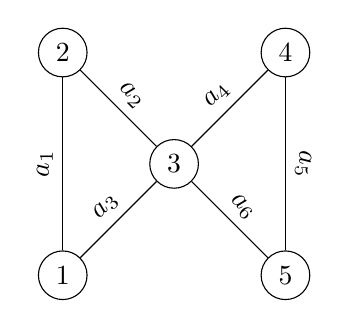
\begin{tikzpicture}[node distance={20mm}, main/.style = {draw, circle}]
            \node[main] (1) {$2$}; 
            \node[main] (2)[below right of=1] {$3$};
            \node[main] (3)[above right of=2] {$4$};
            \node[main] (4)[below right of=2] {$5$};
            \node[main] (5)[below left of=2] {$1$};
            \draw (1) -- node [ above, midway, sloped] {$a_2$}(2);
            \draw (2) -- node [ above, midway, sloped] {$a_4$}(3);
            \draw (3) -- node [ above, midway, sloped] {$a_5$}(4);
            \draw (4) -- node [ above, midway, sloped] {$a_6$}(2);
            \draw (2) -- node [ above, midway, sloped] {$a_3$}(5);
            \draw (5) -- node [ above, midway, sloped] {$a_1$}(1);
        \end{tikzpicture}\\
        \caption{\bf G}
        \label{exv3:image}
    \end{subfigure}
    \caption{Індуковані підграфи графа {\bf G}}
    \label{EXv1:image}
\end{figure}
\textit{Доведення.}\\
Запишемо характеристичні многочлени для графів $\bf G$ і ${\bf G} - \{5\}$. 
\begin{multline*}
P_{\bf G}(\lambda) = \lambda^5 - (a_1^2+a_2^2+a_3^2+a_4^2+a_5^2+a_6^2)\lambda^3 - 2\lambda^2(a_1a_2a_3 + a_4a_5a_6) + \\
+(a_1^2a_4^2+a_1^2a_5^2+a_2^2a_5^2+a_3^2a_5^2+a_1^2a_6^2)\lambda
+2(a_1a_2a_3a_5^2 +a_4a_5a_6a_1^2)
\end{multline*}
$P_{\bf G-\{5\}}(\lambda) = \lambda^4 - \lambda^2(a_1^2+a_2^2+a_3^2+a_4^2)- 2a_1a_2a_3\lambda + a_1^2a_4^2 $

Спектр ребра (4;5) відновлює $a_5$. Оскільки нам відомо чому дорівнює коефіцієнт $a_1^2+a_2^2+a_3^2+a_4^2$ зі спектра ${\bf G}-\{5\}$ і $a_5$, то з коефіцієнта характеристичного многочлена вихідного графа $a_1^2+a_2^2+a_3^2+a_4^2+a_5^2+a_6^2$ однозначно відновлюємо $a_6$.

Зі спектра ${\bf G}-\{5\}$ відомо чому дорівнює $a_1a_2a_3$. З коефіцієнта $(a_1a_2a_3 + a_4a_5a_6)$ спектра $\bf G$ можемо знайти значення $a_4a_5a_6$. Оскільки нам відомо $a_5$, $a_1a_2a_3$ і $a_4a_5a_6$, з $(a_1a_2a_3a_5^2 +a_4a_5a_6a_1^2)$ однозначно відновлюємо $a_1$.

Оскільки нам відомо $a_1$ з коефіцієнта $a_1^2a_4^2$ однозначно відновлюємо $a_4$.
Для відновлення ваг $a_2,a_3$, треба знати спектр ребра (2;3) або (1;3).Тобто такий набір підспектрів однозначно відновлює ваги вихідного графа метелика.

